\section{Exkurs: Zusammenarbeit und Kommunikation von IT und Fachabteilungen}
\subsection{Exkurs: What You Want Is What You Get}
   
    \begin{frame}
      \frametitle<beamer>{Exkurs: What You Want Is What You Get}
      \begin{quote}
        Herr K. berichtet der KFZ-Werkstatt erregt über sein Ärgernis. Er ist tagtäglich auf einer serpentinenreichen Landstraße unterwegs. In einem unübersichtlichen Streckenteil hoppelt jedes Mal dieser verdammte Hase über die Straße. Da K. Tiere liebt, weicht er instinktiv aus, was bei nassem Fahrbahnbelag dazu führt, dass er unweigerlich ins Rutschen gerät und einen Baum touchiert. Für Schäden an Stoßstange und Karosserie hat er bereits ein halbes Vermögen ausgegeben.
      \end{quote}
    \end{frame}
    \only<article>{
      \begin{quote}
        Werkstattmeister M. nickt verständnisvoll: ``Was kann ich da für Sie tun?''
      \end{quote}
    }
    \begin{frame}
      \begin{quote}
        Herr K. : ``Könnten Sie mir nicht eine zusätzliche Knautschzone an Stoßstange und Karosserie montieren?''
      \end{quote}
      \hfill (Michael Stal, heise.de: ``Der Hase und der Baum'')
    \end{frame}
    
    \only<article>{
      Manche Probleme zwischen Fachabteilungen und IT entstehen durch den Versuch der Fachabteilungen, den richtigen Lösungsansatz vorzugeben. So wird in obigem Beispiel wird keine Anforderung formuliert, sondern bereits ein Lösungsansatz. Dem Auftraggeber fehlt aber technisches Hintergrundwissen, so dass er nicht auf die optimale Lösung kommt.
    
      Anforderungen mit Lösungsansätzen sind vollkommen OK, sofern der Auftraggeber dafür triftige Gründe und das entsprechende technische Wissen hat. 
      }

    \begin{frame}
      \begin{quote}
        Gefährlich sind aber Bezüge auf den Lösungsraum, falls sie von Auftraggebern mit wenig technischem Know-how stammen. \hfill (nochmal Michael Stal, heise.de)
      \end{quote}
    \end{frame}

    \only<article>{
      Ich würde es nicht gleich als ``gefährlich'' bezeichnen, aber wenig zielführend ist es auf jeden Fall. 
    }

    \begin{frame}
      \frametitle<beamer>{Kommunikationskunst}
        \begin{quote}
          Die Kunst besteht darin, der jeweils anderen Seite gewisse Kompetenzen einzuräumen.

          Das gilt sowohl für Fachabteilungen als auch für IT--Abteilungen! \hfill (SK)
        \end{quote}
    \end{frame}

    \only<article>{
      Tatsächlich scheinen Informatiker wie auch Informationswissenschaftler einen eher speziellen Blick auf selbstverständliche Dinge zu haben --- zumindest sieht es für den jeweils anderen so aus, oder? 
    }


  \section{Datenbanksysteme}

    \begin{frame}
      \frametitle{Warum Datenbanken?}
      \begin{itemize}
        \pause
        \item Speicherplatz
        \pause
        \item gleichzeitiger Zugriff durch viele Nutzer
      \end{itemize}
    \end{frame}

    \only<article>{
      Da Speicher früher sehr teuer war, entwickelte man Strategien, um Speicherplatz zu sparen. Ein gutes Beispiel sind Normalisierungen bei relationalen Datenbanken.
      }


    \subsection{relationale Datenbanken}
      \only<article>{
        Nehmen wir zur Verdeutlichung eine Versicherung, die die Adressen ihrer Kunden in einer Datenbank speichern möchte. Es wird eine grosse Tabelle angelegt, je eine Zeile pro Kunde. Dabei stellt sich heraus, dass die Versicherung 1000 Kunden hat, die in der Hauptstrasse wohnen. Das bedeutet, dass wir 1000 Mal den Speicherplatz für das Wort ``Hauptstrasse'' benötigen.}
      
      \begin{frame}
      \frametitle{Eine Kundentabelle}
        \begin{center}
          \begin{tabular}{lllll}
            id & Nachname & Vorname & Strasse & Stadt\\
            \hline
            1 & Muster & Hans & Hauptstrasse & Zürich\\
            2 & Meier & Heinrich & Hauptstrasse & Zürich\\
            3 & Müller & Hubert & Hauptstrasse & Zürich\\
            4 & Schulze & Herbert & Hauptstrasse & Zürich\\
          \end{tabular}
        \end{center}
      \end{frame}

        \only<article>{
          Wenn man nun die Strassen in eine extra Tabelle schreibt, eine Zeile pro Strasse, dann muss man in der Tabelle der Kunden nur die ID der Strasse hinterlegen. Wenn die Hauptstrasse z.B. die ID 1 hat, dann benötigen wir nur noch 1000 Mail den Speicherplatz für den Integer 1 --- wesentlich weniger, als für den String ``Hauptstrasse''. Analog kann man z.B. auch mit Städten verfahren. 
        }

      \begin{frame}
      \frametitle{Tabelle der Strassen}
        \begin{center}
          \begin{tabular}{ll}
            id & Strasse\\
            \hline
            1 & Hauptstrasse\\
            2 & Nebenstrasse\\
            3 & Seitenstrasse\\
          \end{tabular}
        \end{center}
      \end{frame}

      \begin{frame}
      \frametitle{Tabelle der Städte}
        \begin{center}
          \begin{tabular}{ll}
            id & Stadt\\
            \hline
            1 & Zürich\\
            2 & Basel\\
            3 & Bern\\
          \end{tabular}
        \end{center}
      \end{frame}

      \begin{frame}
      \frametitle{Tabelle mit Relationen}
        \begin{center}
          \begin{tabular}{lllcc}
            id & Nachname & Vorname & Strassen\_ID & Stadt\_ID\\
            \hline
            1 & Muster & Hans & 1 & 1\\
            2 & Meier & Heinrich & 1 & 1\\
            3 & Müller & Hubert & 1 & 1\\
            4 & Schulze & Herbert & 1 & 1\\
          \end{tabular}
        \end{center}
      \end{frame}

      \begin{frame}
      \frametitle{Speicherplatzbedarf}
          \begin{center}
            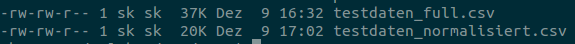
\includegraphics[width=0.8\textwidth]{pics/speicherplatzbedarf}
          \end{center}
      \end{frame}
      
        \only<article>{
          Eine relationale Datenbank dahingehend zu optimieren, dass es möglichst wenig Redundanzen gibt, nennt man ``normalisieren''. Es gibt fünf Normalformen, und für die Datenbank--Spezialisten war es eine komplexe Aufgabe, Daten optimal zu normalisieren.
      
          Die Normalisierung hat auch Nachteile. So liegen nicht alle Informationen in einer Tabelle, was Abfragen komplexer macht. Damit einher geht ein höherer Leistungsbedarf des Servers.
        }

    \begin{frame}
    \frametitle<beamer>{Relationen in der DB von Aleph}
      \begin{figure}
        \begin{center}
          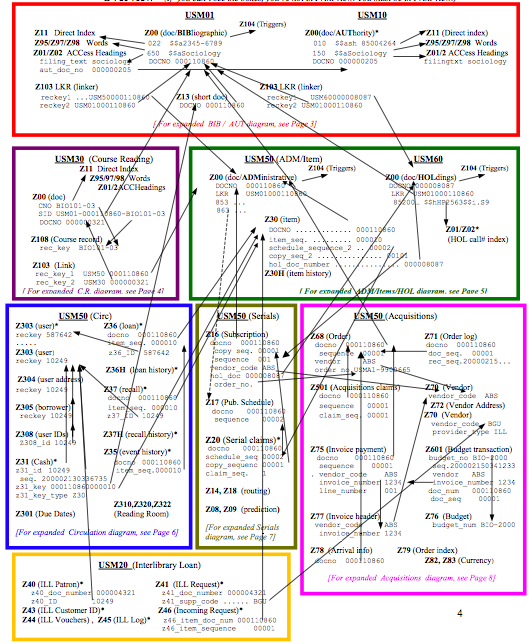
\includegraphics[width=0.4\textwidth]{pics/alephtables}
            \only<article>{\caption{Relationen in der DB von Aleph}}
          \end{center}
        \end{figure}
    \end{frame}

\begin{frame}[fragile]
\frametitle{Felder nicht atomar}
  \begin{lstlisting}
    select substr(z103_rec_key,6,9) || 'EHO60'
    from eho60.z103
    where substr(z103_lkr_text_n,1,3) = 'E04'
    and z103_lkr_library = 'EBI01'
    and substr(z103_rec_key,1,5) = 'EHO60'
    ;
  \end{lstlisting}
\end{frame}
        
        \only<article>{
          Ein Nachteil von relationalen Datenbanken ist die feste Grösse und Anzahl von Feldern. Wenn ich beispielsweise für die Tabelle der Kunden die Spalten
      
          \begin{tabular}{rrrrrr}
            Vorname & Nachname & Strasse & Hausnummer & Postleitzahl & Ort\\
          \end{tabular}
      
          festgelegt habe, und die Versicherung sich entscheidet, ein internationales Geschäft aufzubauen, ist es einiger Aufwand, die Spalte ``Land'' hinzu zu fügen.
        }

      \begin{frame}
        \frametitle{feste Grösse}
        Das Feld für Inventarnummern darf in Aleph nicht mehr als 20 Zeichen haben. 
      \end{frame}

      \begin{frame}
      \frametitle{und wieder: Kodierung von Text}
        \begin{quote}
          UTF8-Codierungszeichen zaehlen einzeln, auch wenn daraus ein einziges Unicode-Zeichen entsteht. 

          Ein Beispiel dafuer ist das ``Ä'', das im Inventarnummernfeld zwei VARCHAR2 Zeichen aufbraucht, weil es aus 0xc3 und 0x84 besteht. 

          Ich habe nicht geschaut, ob es noch weitere solche Fälle gibt. \hfill{[Mathias Weyland]}
        \end{quote}
      \end{frame}

    \subsection{dokumentorientierte Datenbanken}
      \begin{frame}
        \frametitle<beamer>{dokumentorientierte Datenbanken}
        \begin{center}
          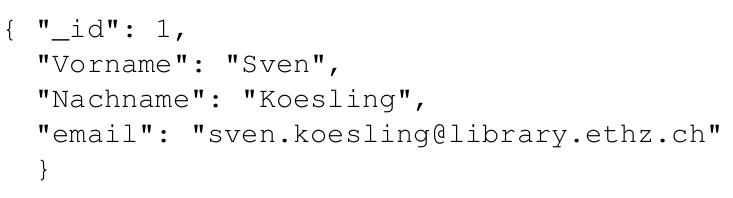
\includegraphics[width=0.8\textwidth]{pics/doc1}
        \end{center}
      \end{frame}

      \begin{frame}
        \frametitle{ein weiteres Dokument in derselben collection}
        \begin{center}
        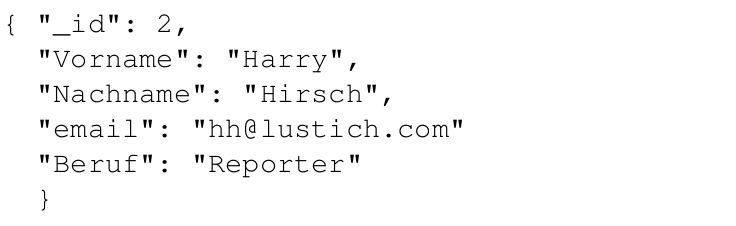
\includegraphics[width=0.8\textwidth]{pics/doc2}
        \end{center}
      \end{frame}
      
      \begin{frame}
        \frametitle{noch ein Dokument in derselben collection}
        \begin{center}
        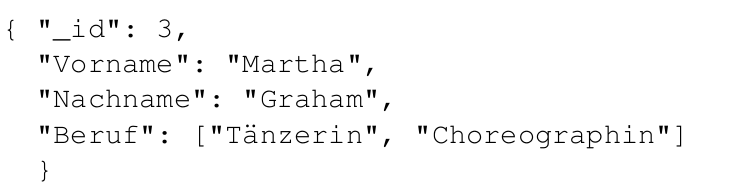
\includegraphics[width=0.8\textwidth]{pics/doc3}
        \end{center}
      \end{frame}

      \begin{frame}
        \frametitle{und noch ein weiteres Dokument in derselben collection}
        \begin{center}
        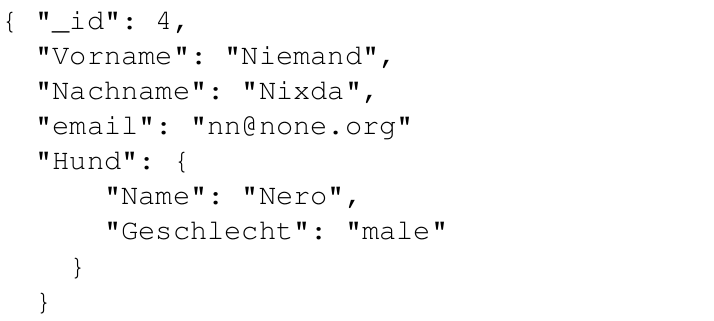
\includegraphics[width=0.8\textwidth]{pics/doc4}
        \end{center}
      \end{frame}

    \subsection{Abstraktion}

    \subsection{Indexer}
      \begin{frame}
        \begin{figure}
          \caption{Suche nach ``Landquart'' in einem aktuellen Bibliothekskatalog (420.000 Dokumente): 1072 Treffer -- ohne Facetten: completed in 2845ms}
          \begin{center}
            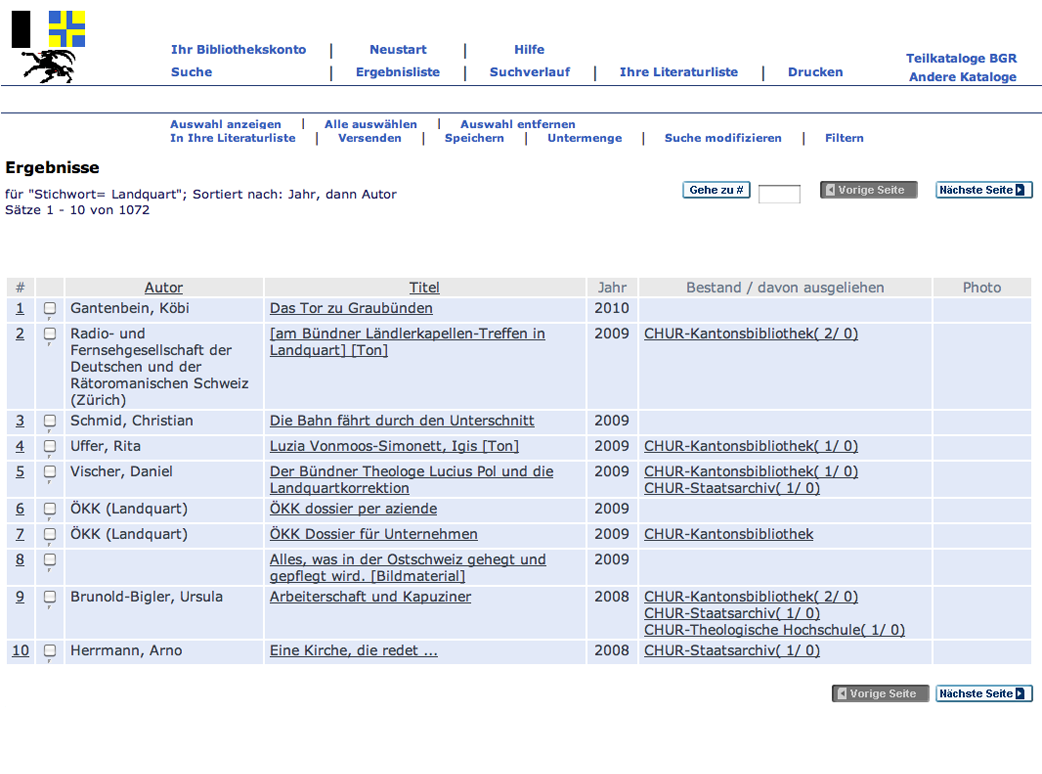
\includegraphics[width=0.8\textwidth]{pics/aleph}
          \end{center}
        \end{figure}
      \end{frame}

      \begin{frame}
        \begin{figure}
          \caption{Die gleiche Suche mit einem Indexer: 1.700 Treffer mit drei Facetten: completed in 792ms}
          \begin{center}
            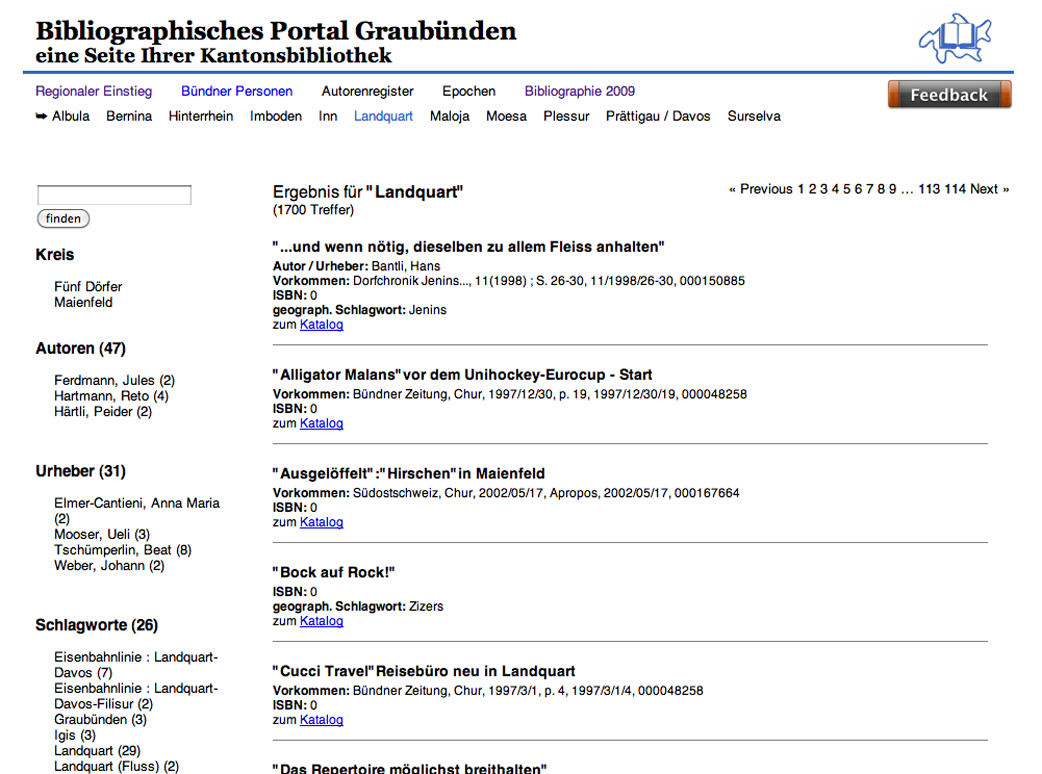
\includegraphics[width=0.8\textwidth]{pics/Ergebnis}
          \end{center}
        \end{figure}
      \end{frame}